\documentclass[12pt]{article}

\usepackage[spanish]{babel}
\usepackage[none]{hyphenat}
\usepackage[left=1.5cm, right=1.5cm, top = 2cm, bottom=2.5cm]{geometry}
\usepackage{parskip}
\usepackage[export]{adjustbox}
\usepackage{enumitem}[shortlabels]
\usepackage{listings} 
\usepackage{color}
\usepackage{fancyhdr}
\usepackage{graphicx}
\usepackage{caption} 
% \usepackage{subcaption}
\usepackage{wrapfig}
% \usepackage{longtable}
% \usepackage{multirow, makecell}
% \usepackage{amsmath} 
\usepackage[hidelinks]{hyperref}
\usepackage{csquotes}
% \usepackage{tocloft}

\newcommand{\linejump}{\hfill \break}
\renewcommand{\thefootnote}{\fnsymbol{footnote}}
% \newcommand{\unit}[1]{\ensuremath{\, \mathrm{#1}}}

\definecolor{dkgreen}{rgb}{0,0.6,0}
\definecolor{gray}{rgb}{0.5,0.5,0.5}
\definecolor{mauve}{rgb}{0.58,0,0.82}
\lstset{
  language=Java,
  aboveskip=3mm,
  belowskip=3mm,
  showstringspaces=false,
  columns=flexible,
  basicstyle={\scriptsize\ttfamily},
  numbers=none,
  numberstyle=\tiny\color{gray},
  keywordstyle=\color{blue},
  commentstyle=\color{dkgreen},
  stringstyle=\color{mauve},
  breaklines=true,
  breakatwhitespace=true,
  tabsize=2
}

\sloppy
\setlength{\parindent}{0cm}
\setlength{\columnsep}{0.5cm}
\decimalpoint
\graphicspath{{img/}}

\hypersetup{colorlinks=true, urlcolor=blue, citecolor=blue}
\urlstyle{same}

\pagestyle{fancyplain}
\fancyhf{}
\fancyhead[L]{\scriptsize 
  Universidad Nacional Autónoma de México \\
  Programación Orientada a Objetos \\
  M.C. Leonardo Ledesma Dominguez
}
\fancyhead[R]{\thepage}


\begin{document}
  \begin{center}
    Acosta Porcayo Alan Omar 320206102, Luna Valdin Uriel 320293256 \\
    \linejump
    \LARGE \textbf{Tarea 7. Manejo de excepciones}
  \end{center}
  
  \linejump
  \begin{enumerate}
    \item Realice un cuadro sinóptico de excepciones y errores indicando:
    \begin{enumerate}[label=\alph*.]
      \item Excepciones
      \begin{enumerate}[label=\roman*.]
        \item Marcadas (Tiempo de compilación)
        \item No Marcadas (Tiempo de ejecución)
      \end{enumerate}
      \item Errores
      \begin{enumerate}[label=\roman*.]
        \item Sintácticos (Tiempo de compilación)
        \item Semánticos (Tiempo de ejecución)
      \end{enumerate}
    \end{enumerate}

    \begin{figure}[h!]
      \centering
      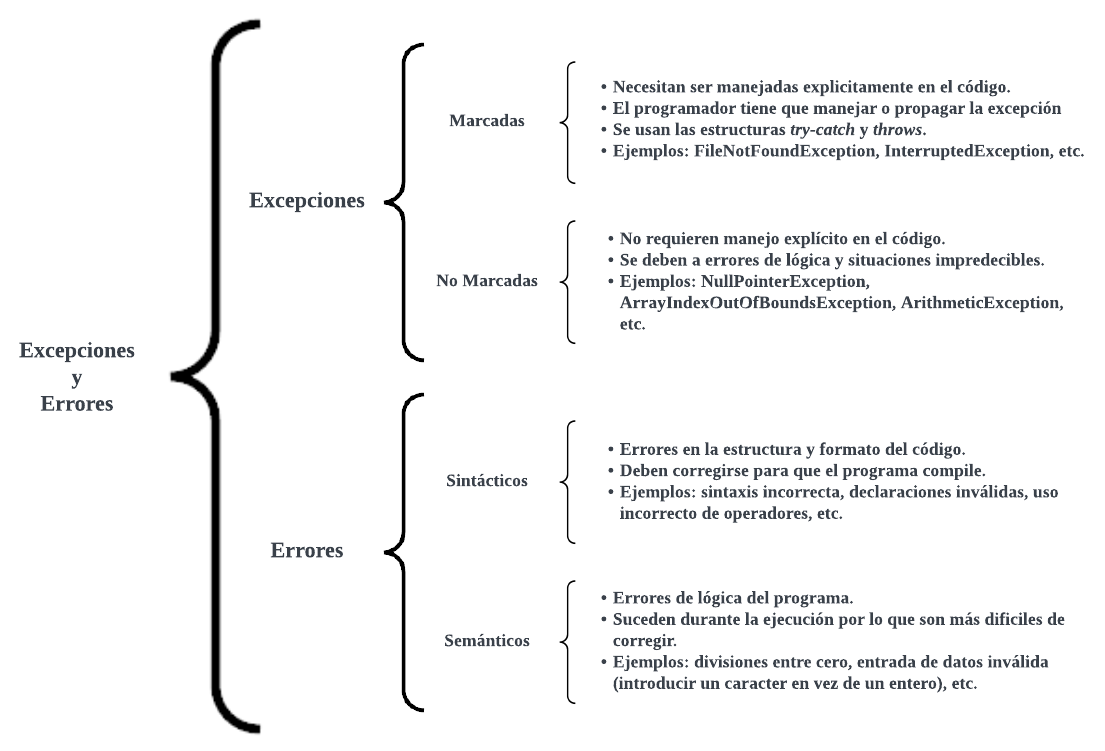
\includegraphics[width=0.9\textwidth]{sinoptico.png}
    \end{figure}

    \newpage
    \item Realice una tabla comparativa entre el uso de las palabras reservadas \textit{throw} y \textit{throws}.
    
    \begin{table}[h!]
      \centering
      \begin{tabular}{|p{0.45\textwidth}|p{0.45\textwidth}|}
        \hline
        \begin{center} \textbf{\textit{throw}} \end{center} & \begin{center} \textbf{\textit{throws}} \end{center} \\ \hline 
        Se utiliza para lanzar una excepción explícitamente en el código. & Se usa en la declaración de un método para indicar que en alguna parte del código puede ocurrir esa excepción. \\ \hline
        Solo se pueden propagar excepciones no marcadas. & Solo se pueden propagar excepciones marcadas. \\ \hline
        La palabra reservada \textit{throw} se usa dentro del cuerpo del método. & La palabra reservada \textit{throws} se usa en la declaración del método. \\ \hline
        Después de la palabra reservada \textit{throw} se debe especificar una instancia de la clase \textit{Throwable} o una subclase de esta. & Después de la palabra reservada \textit{throws} se debe especificar una clase que extienda de \textit{Throwable}. \\ \hline
        Se puede lanzar una excepción a la vez. & Se pueden lanzar varias excepciones a la vez. \\ \hline
      \end{tabular}
    \end{table}

    \item Realice un programa ocupando interfaces y clases abstractas implementando al menos una excepción usando:
    \begin{enumerate}[label=\alph*.]
      \item \textit{try catch} - operación no válida
      \item \textit{try catch resources} - Tarjeta de debido/crédito no válida
      \item \textit{throw} - excepción propia sin saldo suficiente
      \item \textit{throws} - NIP incorrecto
    \end{enumerate}
    El programa simula un ATM considere las clases Banco (interfaz), ATM (clase concreta) que implementa a Banco, Tarjeta (clase abstracta), Tarjeta de débito / crédito hereda de Tarjeta (clase concreta) y Cliente(clase concreta). Considere que las opciones del cliente pueden hacer retirar, abonar y consultar saldo, así como el ATM, de disminuir /aumentar saldo, verificar saldo, verificar NIP.

    \textbf{\textit{Banco.java}}
    \begin{lstlisting}
public interface Banco{

	void retirar(double cantidad) throws OperacionNoValidaException; 
	void abonar(double cantidad) throws OperacionNoValidaException; 
	double consultarSaldo();
	 
}
    \end{lstlisting}

    \textbf{\textit{ATM.java}}
    \begin{lstlisting}
class ATM implements Banco {
  private double saldoATM;

  public ATM(double saldoInicialATM) {
    this.saldoATM = saldoInicialATM;
  }

  @Override
  public void retirar(double cantidad) throws OperacionNoValidaException {
    if (cantidad <= 0 || cantidad > saldoATM) {
      throw new OperacionNoValidaException("Operacion de retiro no valida en el ATM");
    }
    saldoATM -= cantidad;
    System.out.println("Retiro exitoso en el ATM. Nuevo saldo del ATM: " + saldoATM);
  }

  @Override
  public void abonar(double cantidad) throws OperacionNoValidaException {
    throw new OperacionNoValidaException("Operacion de abono no permitida en el ATM");
  }

  @Override
  public double consultarSaldo() {
      return saldoATM;
  }

  // Metodo para verificar saldo en la tarjeta
  public void verificarSaldoTarjeta(Tarjeta tarjeta) throws OperacionNoValidaException {
    if (tarjeta.consultarSaldo() <= 0) {
      throw new OperacionNoValidaException("Saldo insuficiente en la tarjeta");
    }
  }
}
    \end{lstlisting}

    \textbf{\textit{Tarjeta.java}}
    \begin{lstlisting}
import java.util.HashSet;
import java.util.Set;


public abstract class Tarjeta {
  protected double saldo;
  protected Set<Integer> nipsUtilizados;

  public Tarjeta(double saldoInicial) {
    this.saldo = saldoInicial;
    this.nipsUtilizados = new HashSet<>();
  }

  public abstract void verificarNIP(int nip) throws NIPIncorrectoException;

  public double consultarSaldo() {
    return saldo;
  }
}

class TarjetaDebito extends Tarjeta {
  private int nip;

  public TarjetaDebito(double saldoInicial, int nip) {
    super(saldoInicial);
    this.nip = nip;
  }

  @Override
  public void verificarNIP(int nipIngresado) throws NIPIncorrectoException {
    if (nipIngresado != nip) {
      throw new NIPIncorrectoException("NIP incorrecto");
    }
  }
}

class TarjetaCredito extends Tarjeta {
  private int nip;

  public TarjetaCredito(double saldoInicial, int nip) {
    super(saldoInicial);
    this.nip = nip;
  }

  @Override
  public void verificarNIP(int nipIngresado) throws NIPIncorrectoException {
    if (nipIngresado != nip) {
      throw new NIPIncorrectoException("NIP incorrecto");
    }
  }
}
    \end{lstlisting}

    \textbf{\textit{Cliente.java}}
    \begin{lstlisting}
class Cliente implements Banco {
  private String nombre;
  private Tarjeta tarjeta;

  public Cliente(String nombre, Tarjeta tarjeta) {
    this.nombre = nombre;
    this.tarjeta = tarjeta;
  }

  @Override
  public void retirar(double cantidad) throws OperacionNoValidaException {
    if (cantidad <= 0 || cantidad > tarjeta.consultarSaldo()) {
      throw new OperacionNoValidaException("Operacion de retiro no valida");
    }
    tarjeta.saldo -= cantidad;
    System.out.println("Retiro exitoso. Nuevo saldo: " + tarjeta.consultarSaldo());
  }

  @Override
  public void abonar(double cantidad) throws OperacionNoValidaException {
    if (cantidad <= 0) {
      throw new OperacionNoValidaException("Operacion de abono no valida");
    }
    tarjeta.saldo += cantidad;
    System.out.println("Abono exitoso. Nuevo saldo: " + tarjeta.consultarSaldo());
  }

  @Override
  public double consultarSaldo() {
    return tarjeta.consultarSaldo();
  }

  public Tarjeta getTarjeta() {
    return tarjeta;
  }
}
    \end{lstlisting}

    \textbf{\textit{OperacionNoValidaException.java}}
    \begin{lstlisting}
class OperacionNoValidaException extends Exception{
	
	public OperacionNoValidaException(String mensaje){
		super(mensaje);
	}

}
    \end{lstlisting}

    \textbf{\textit{NIPIncorrectoException.java}}
    \begin{lstlisting}
class NIPIncorrectoException extends Exception {

  public NIPIncorrectoException(String mensaje) {
    super(mensaje);
  }
    
}
    \end{lstlisting}

    \textbf{\textit{ProgramaATM.java}}
    \begin{lstlisting}
import java.util.HashMap;
import java.util.Map;
import java.util.Scanner;


public class ProgramaATM {
  private static Map<String, Cliente> clientesRegistrados = new HashMap<>();

  public static void main(String[] args) {
    Scanner scanner = new Scanner(System.in);

    // Menu principal
    int opcion;
    do {
      System.out.println("\n\n\t ATM -/ENGINEERS/- ");
      System.out.println("1. Crear cuenta");
      System.out.println("2. Ingresar a la cuenta");
      System.out.println("3. Salir");
      System.out.print("Ingrese su opcion: ");
      opcion = scanner.nextInt();

      switch (opcion) {
        case 1:
          crearCuenta(scanner);
          break;
        case 2:
          ingresarCuenta(scanner);
          break;
        case 3:
          System.out.println("Saliendo del programa. Hasta luego!");
          break;
        default:
          System.out.println("Opcion no valida. Por favor, ingrese una opcion valida.");
      }
    } while (opcion != 3);

    scanner.close();
  }

  private static void crearCuenta(Scanner scanner) {
    System.out.println("\nSeleccione el tipo de tarjeta:");
    System.out.println("1. Tarjeta de Debito");
    System.out.println("2. Tarjeta de Credito");
    System.out.print("Ingrese su opcion: ");
    int tipoTarjeta = scanner.nextInt();

    scanner.nextLine(); 

    System.out.print("Ingrese su nombre: ");
    String nombre = scanner.nextLine();

    if (clientesRegistrados.containsKey(nombre)) {
      System.out.println("Este usuario ya ha sido creado.");
      return;
    }

    System.out.print("Ingrese su NIP: ");
    int nip = scanner.nextInt();

    Tarjeta tarjeta;
    if (tipoTarjeta == 1) {
      tarjeta = new TarjetaDebito(0, nip); 
    } else if (tipoTarjeta == 2) {
      tarjeta = new TarjetaCredito(5000, nip); 
    } else {
      System.out.println("Opcion no valida. La cuenta no fue creada.");
      return;
    }

    try {
      tarjeta.verificarNIP(nip);
      Cliente nuevoCliente = new Cliente(nombre, tarjeta);
      clientesRegistrados.put(nombre, nuevoCliente);
      System.out.println("Usuario registrado con exito.");
    } catch (NIPIncorrectoException e) {
      System.out.println("Error: " + e.getMessage());
    }
  }


  private static void ingresarCuenta(Scanner scanner) {
    System.out.print("\nIngrese su nombre: ");
    String nombre = scanner.next();

    if (clientesRegistrados.containsKey(nombre)) {
      Cliente cliente = clientesRegistrados.get(nombre);
      System.out.print("Ingrese su NIP: ");
      int nip = scanner.nextInt();
      try {
        cliente.getTarjeta().verificarNIP(nip);
        menuOperaciones(scanner, cliente);
      } catch (NIPIncorrectoException e) {
        System.out.println("Error: " + e.getMessage());
      }
    } else {
      System.out.println("Usuario no registrado. Por favor, cree una cuenta primero.");
    }
  }


  private static void menuOperaciones(Scanner scanner, Cliente cliente) {
    int opcion;
    do {
      System.out.println("\n1. Retirar");
      System.out.println("2. Abonar");
      System.out.println("3. Consultar saldo");
      System.out.println("4. Salir");
      System.out.print("Ingrese su opcion: ");
      opcion = scanner.nextInt();

      switch (opcion) {
        case 1:
          System.out.print("\nIngrese la cantidad a retirar: ");
          double cantidadRetiro = scanner.nextDouble();
          try {
            cliente.retirar(cantidadRetiro);
          } catch (OperacionNoValidaException e) {
            System.out.println("Error: " + e.getMessage());
          }
          break;
        case 2:
          System.out.print("\nIngrese la cantidad a abonar: ");
          double cantidadAbono = scanner.nextDouble();
          try {
            cliente.abonar(cantidadAbono);
          } catch (OperacionNoValidaException e) {
            System.out.println("Error: " + e.getMessage());
          }
          break;
        case 3:
          System.out.println("Saldo actual: " + cliente.consultarSaldo());
          break;
        case 4:
          System.out.println("Saliendo del menu de operaciones.");
          break;
        default:
          System.out.println("Opcion no valida. Por favor, ingrese una opcion valida.");
      }
    } while (opcion != 4);
  }
}
    \end{lstlisting}

    \textbf{Ejemplo de ejecución:}
    \begin{figure}[h!]
      \centering
      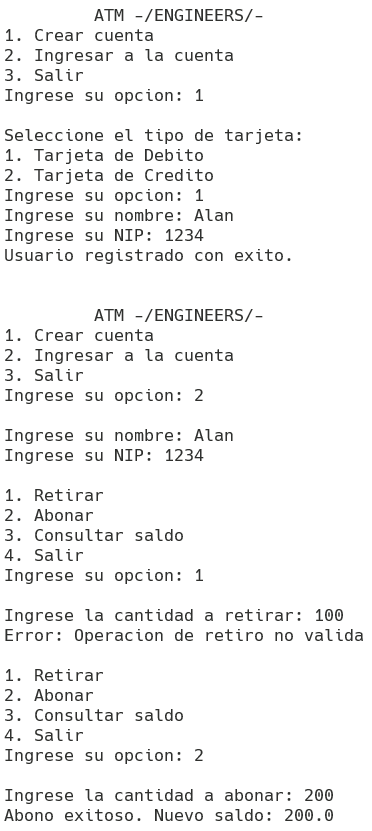
\includegraphics[width=0.45\textwidth]{ATM.png}
    \end{figure}

    \item Lea y haga un resumen del capitulo 2 del libro que el profesor compartió en classroom de Richard Warburton: ``\textit{JAVA 8 Lambdas}''.
    
    La introducción de expresiones lambda en Java 8 marca un hito significativo en la evolución del lenguaje. Estas expresiones proporcionan una forma concisa de incorporar comportamientos directamente en el código, representando un componente esencial que define el paradigma de programación funcional en Java. Para comprender la utilidad de las expresiones lambda, observemos un escenario común en la programación de interfaces gráficas de usuario (GUI) con la biblioteca Swing de Java. Tradicionalmente, para manejar eventos como clics de botón, se utilizan clases internas anónimas, lo que lleva a un código con un exceso de boilerplate.

    \begin{lstlisting}[basicstyle={\normalsize\ttfamily}]
button.addActionListener(new ActionListener() {
  public void actionPerformed(ActionEvent event) {
    System.out.println("Boton clickeado");
  }
});
    \end{lstlisting}

    Sin embargo, las clases internas anónimas no ofrecen una solución eficiente para pasar código como datos. Además del código redundante, la intención del programador se ve opacada. En Java 8, la introducción de expresiones lambda aborda esta problemática, permitiendo escribir el mismo código de manera más clara y concisa:

    \begin{lstlisting}[basicstyle={\normalsize\ttfamily}]
button.addActionListener(event -> System.out.println("Boton clickeado"));
    \end{lstlisting}

    Aquí, en lugar de pasar un objeto que implementa una interfaz, se envía un bloque de código, una función anónima. La variable event actúa como un parámetro, y -> separa dicho parámetro del cuerpo de la expresión lambda, que representa el código ejecutado al hacer clic en el botón.

    Una diferencia clave entre el enfoque tradicional y el uso de expresiones lambda radica en cómo se declara la variable event. Antes, era necesario especificar explícitamente su tipo: ActionEvent event. En el ejemplo con expresiones lambda, la declaración de tipo se omite, y el compilador infiere el tipo desde el contexto, como en la firma de addActionListener. Este proceso, conocido como inferencia de tipos, elimina la necesidad de declaraciones explícitas cuando el tipo es obvio.

    \begin{lstlisting}[basicstyle={\normalsize\ttfamily}]
Runnable sinArgumentos = () -> System.out.println("Hola Mundo");

ActionListener unArgumento = event -> System.out.println("Boton clickeado");

Runnable multiLinea = () -> {
  System.out.print("Hola");
  System.out.println(" Mundo");
};

BinaryOperator<Long> suma = (x, y) -> x + y;

BinaryOperator<Long> sumaExplicita = (Long x, Long y) -> x + y;
    \end{lstlisting}

    Las expresiones lambda admiten diversas formas de sintaxis, lo que brinda flexibilidad al programador. Pueden ser sin argumentos, con un solo argumento, con bloques de código multilineales o con múltiples argumentos, Las interfaces funcionales desempeñan un papel central en la utilización efectiva de expresiones lambda. Una interfaz funcional es aquella con un único método abstracto y se convierte en el tipo de una expresión lambda que implementa dicho método. La interfaz funcional ActionListener, presente en el ejemplo, tiene un solo método, actionPerformed, y puede ser sustituida por una expresión lambda.

    Estas interfaces permiten dar un nombre significativo al tipo del parámetro, mejorando la legibilidad del código. La inferencia de tipos también es crucial aquí; el compilador puede adaptar automáticamente el tipo del parámetro según el contexto. En situaciones específicas, puede ser necesario proporcionar pistas de tipo manualmente. La recomendación es seguir la práctica que facilite la lectura del código, ya sea omitiendo tipos para reducir el ruido visual o incluyéndolos para mayor claridad. La decisión puede basarse en reglas simples que se detallarán más adelante en este capítulo.

    La introducción de expresiones lambda y la inferencia de tipos en Java 8 representa un cambio fundamental en la forma en que los programadores abordan el diseño y la estructuración del código. La flexibilidad sintáctica y la potencia de las interfaces funcionales y las expresiones lambda allanan el camino para un estilo de programación más conciso y expresivo. Estas herramientas fundamentales sientan las bases para explorar conceptos avanzados en programación funcional.
  \end{enumerate}

  \section*{Referencias}
  \textit{Difference between throw and throws in java - javatpoint}. (2021). www.javatpoint.com. \url{https://www.javatpoint.com/difference-between-throw-and-throws-in-java} \\

  Warburton, R. (2014). \textit{Java 8 lambdas: Functionnal Programming for the Masses}. Oreilly $\&$ Associates Incorporated.
\end{document}